% !TEX TS-program = pdflatex
% !TEX encoding = UTF-8 Unicode

% This is a simple template for a LaTeX document using the "article" class.
% See "book", "report", "letter" for other types of document.

\documentclass[10pt,twocolumn]{article}

\usepackage[utf8]{inputenc} % set input encoding (not needed with XeLaTeX)
\usepackage{graphicx}
\usepackage{listings} 
\usepackage{xcolor,colortbl}
\usepackage[section]{placeins}
\usepackage{amsthm}
\usepackage{mathtools}
\graphicspath{ {images/} }

%%% Examples of Article customizations
% These packages are optional, depending whether you want the features they provide.
% See the LaTeX Companion or other references for full information.

%%% PAGE DIMENSIONS
\usepackage{geometry} % to change the page dimensions
\geometry{a4paper} % or letterpaper (US) or a5paper or....
\geometry{margin=0.55in} % for example, change the margins to 2 inches all round
% \geometry{landscape} % set up the page for landscape
%   read geometry.pdf for detailed page layout information

\usepackage{graphicx} % support the \includegraphics command and options

% \usepackage[parfill]{parskip} % Activate to begin paragraphs with an empty line rather than an indent

%%% PACKAGES
\usepackage{booktabs} % for much better looking tables
\usepackage{array} % for better arrays (eg matrices) in maths
\usepackage{paralist} % very flexible & customisable lists (eg. enumerate/itemize, etc.)
\usepackage{verbatim} % adds environment for commenting out blocks of text & for better verbatim
\usepackage{subfig} % make it possible to include more than one captioned figure/table in a single float
\usepackage{indentfirst}
\usepackage{amsfonts}
\usepackage{amssymb}
\usepackage{amsthm}
% These packages are all incorporated in the memoir class to one degree or another...

%%% HEADERS & FOOTERS
\usepackage{fancyhdr} % This should be set AFTER setting up the page geometry
\pagestyle{fancy} % options: empty , plain , fancy
\renewcommand{\headrulewidth}{0pt} % customise the layout...
\lhead{}\chead{}\rhead{}
\lfoot{}\cfoot{\thepage}\rfoot{}

%%% SECTION TITLE APPEARANCE
\usepackage{sectsty}
\allsectionsfont{\sffamily\mdseries\upshape} % (See the fntguide.pdf for font help)
% (This matches ConTeXt defaults)

%%% ToC (table of contents) APPEARANCE
\usepackage[nottoc,notlof,notlot]{tocbibind} % Put the bibliography in the ToC
\usepackage[titles,subfigure]{tocloft} % Alter the style of the Table of Contents
\renewcommand{\cftsecfont}{\rmfamily\mdseries\upshape}
\renewcommand{\cftsecpagefont}{\rmfamily\mdseries\upshape} % No bold!
\setlength{\parindent}{0.5cm} 

%%% END Article customizations

%%% The "real" document content comes below...

\title{On 6k $\pm$ 1 Primes in Goldbach Strong Conjecture}
\author{Marcin Barylski}
\date{\small{Published: February 18, 2018 \\ The last update: September 3, 2019}}

\definecolor{Gray}{gray}{0.85}
\definecolor{LightCyan}{rgb}{0.88,1,1}
\newcolumntype{a}{>{\columncolor{Gray}}c}
\newcolumntype{b}{>{\columncolor{white}}c}

\newtheorem{theorem}{Theorem}
\newtheorem{lemma}[theorem]{Lemma}

\newcommand\bigforall{\mbox{\huge $\mathsurround0pt\forall$}} 
\newcommand\bigexists{\mbox{\huge $\mathsurround0pt\exists$}} 

\begin{document}
\maketitle

\begin{abstract}
Goldbach strong conjecture, still unsolved, states that all even integers $n \textgreater 2$ can be expressed as the sum of two prime numbers (Goldbach partitions of $n$). Each prime $p \textgreater 3$ can be expressed as $6k \pm 1$. This work is devoted to studies of $6k \pm 1$ primes in Goldbach partitions and enhanced Goldbach strong conjecture with the lesser of twin primes of form $6k - 1$ used as a baseline.
\end{abstract}

\section{Introduction}

Goldbach strong conjecture ($GSC$, also called binary) asserts that all positive even integer $n$ $\geq$ 4 can be expressed as the sum of two prime numbers. This hypothesis, formulated by Goldbach in 1742 in letter to Euler \cite{goldbach1742} and then updated by Euler to the form above is one of the oldest and still unsolved problems in number theory. Empirical verification showed that it is true for all $n$ $\leq$ 4 x $10^{18}$ \cite{oliveira2012} \cite{oliveira2013}.\par
The expression of a given positive even number $n$ as a sum of two primes $p_1$ and $p_2$ is called a Goldbach Partition ($GP$) of $n$.  Let's denote this relation as $GSC(n, p_1, p_2)$. Then Goldbach strong conjecture can be written as (1):

\begin{equation}
\displaystyle\mathop{\bigforall}_{x \textgreater 1, x \in \mathbb{N}} \displaystyle\mathop{\bigexists}_{p_1, p_2 \in \mathbb{P}} GSC (2x, p_1, p_2)
\end{equation}

\section{6k $\pm$ 1  primes in GSC}

Every prime $p \textgreater 3$ can be written as $6k \pm 1$, where $k \in \mathbb{N}$ (lemma proved in \cite{barylski2018}). There are exactly two primes that are not of form $6k \pm 1$: $2$ and $3$. Prime $2$ is present in one partition only: $GSC(4, 2, 2)$, while prime $p = 3$ plays much important role in $GSC$ - it is the most frequent prime in the partitions for even $n \textless 10^6$ \cite{barylski2018}. \par
Let's exclude both primes $2$ and $3$ from a set of primes used to fulfill $GSC$. All remaining primes are of form $6k \pm 1$. It would not be possible to build neither $4$ nor $6$ nor $8$ from a sum of two such primes (because these numbers always have $GP$ with either $2$ or $3$: $GSC(4, 2, 2)$, $GSC(6, 3, 3)$, $GSC(8, 3, 5)$, $GSC(8, 5, 3)$), but situation is changing for bigger even numbers. Let $R(n)$ be a set of $GPs$ of $n$, while  $R_{6k \pm 1}(n)$ a set of $GPs$ of $n$ but without using primes $2$ and $3$ in any $GP$. As shown above: $R_{6k \pm 1}(4) = \emptyset$, $R_{6k \pm 1}(6) = \emptyset$, $R_{6k \pm 1}(8) = \emptyset$.

\begin{lemma}
$0 \leq \left\vert R(n)\right\vert - \left\vert R_{6k \pm 1}(n)\right\vert \leq 1$
\end{lemma}
\begin{proof}
There are exactly two primes $2$ and $3$ that are not of form $6k \pm 1$, where $k \in \mathbb{N}$. Let's analyze two cases: $n = 4$ and $n \textgreater 4$. For first case we have: $R(4) = (2,2)$, $R_{6k \pm 1}(4) = \emptyset$, thus $\left\vert R(4)\right\vert - \left\vert R_{6k \pm 1}(4)\right\vert = 1$ which fulfills the lemma. $2$ is not a part of any other $GP$. Let's take a look at even $n \textgreater 4$. There are $n$ for which $3$ is present in $GP$ (i.e. $R(22) = (3,19), (5,17), (11,11)$, $R_{6k \pm 1}(22) = (5,17), (11,11)$ ) or missing (i.e. $R(24) = R_{6k \pm 1}(24) = (5,19), (7,17), (11,13)$. $3$ can exist in at least one $GP$ for $n \textgreater 4$ because in $GSC(n, 3, p_1)$ we have just one way to express $p_1$: $p_1 = n - 3$. Thus for $n \textgreater 4$ we have that $\left\vert R(n)\right\vert - \left\vert R_{6k \pm 1}(n)\right\vert$ is either $0$ or $1$, and this fulfills the remaining part of the lemma.
\end{proof}

 Let $R_{6k + 1}(n)$ be a set of GPs of $n$ that both factors are primes of form $6k + 1$, and $R_{6k - 1}(n)$ be a set of GPs of $n$ that both factors are primes of form $6k - 1$. By definition $R_{6k + 1}(n) \subseteq R_{6k \pm 1}(n)$ and $R_{6k - 1}(n) \subseteq R_{6k \pm 1}(n)$.

\begin{lemma}
\begin{equation}
\displaystyle\mathop{\bigforall}_{n \in \mathbb{N}}
\left\vert R_{6k - 1}(6n) \right\vert = \left\vert R_{6k + 1}(6n) \right\vert = 0
\end{equation}
\end{lemma}
\begin{proof}
Every number of form $6n$, $n \in \mathbb{N}$, is divisible by both $2$ and $3$. Let's assume that $p_1$ is of form $6k_1-1$ and $p_2$ is of form $6k_2-1$ ($k_1, k_2 \in \mathbb{N}$). Then $s = p_1 + p_2 = 6k_1 - 1 + 6k_2 - 1 = 6(k_1 + k_2) - 2 = 2(3k_1 + 3k_2 - 1)$. $s$ is divisible by $2$ but is not divisible by $3$ because $3$ does not divide $3k_1 + 3k_2 - 1$. Similar reasoning can be done for a case when both $p_1$ and $p_2$ are of form $6k+1$. This means that $6n$ cannot be built from a sum of neither two primes of form $6k-1$ nor $6k+1$.
\end{proof}

\section{GSC broken down into three}

Original $GSC$ does not say anything particular about primes. Let's take a look at even numbers $n \textgreater 8$. Each such number can be expressed as either $3x$ or $3x+1$ or $3x+2$, where $x \in \mathbb{N}$. Calculations run for small $n$  show that original $GSC$ can be extended to a form (3):

\begin{equation}
\displaystyle\mathop{\bigforall}_{m \textgreater 4, m \in \mathbb{N}}
\left\{ \begin{array}{ll}
GSC(2m, p_{6k-1}, p_{6k+1}) & \textrm{if $m$ $mod$ $3 = 0$}\\
GSC(2m, p_{6k+1}, p_{6k+1}) & \textrm{if $m$ $mod$ $3 = 1$}\\
GSC(2m, p_{6k-1}, p_{6k-1}) & \textrm{if $m$ $mod$ $3 = 2$}\\
\end{array} \right.
\end{equation}
\\where 
$p_{6k-1}$ is a prime of form ${6a-1}$ \cite{A007528} and $p_{6k+1}$ is a prime of form  ${6b+1}$ \cite{A002476} ($a, b \in \mathbb{N}$). Conjecture (3) uses limited set of prime numbers in $GSC$ - primes $2$ and $3$ are excluded.\par
Every twin prime pair different than $(3, 5)$ is of form ($6k - 1$, $6k + 1$), where $k \in \mathbb{N}$ \cite{barylski2018}. This gives a hint that yet stronger version of conjecture (3) is potentially possible. If we assume that $k$ is the same in all three conditions for the same $n$, and both $p_{6k-1}$ are the lesser of twin primes ($\mathbb{P_{LT}}$), then we can articulate the following  hypothesis (4):

\begin{equation}
\displaystyle\mathop{\bigexists}_{A \in \mathbb{N}}
\displaystyle\mathop{\bigforall}_{n \textgreater A, n \in \mathbb{N}}
\displaystyle\mathop{\bigexists}_{p_1, p_2 \in \mathbb{P_{LT}}}
GSC(6n-2, p_1, p_2)
\end{equation}
\\where 
$A$ is a constant to be provided. 

\begin{lemma}
If conjecture (4) is true, then we have a method to proof or invalidate $GSC$.
\end{lemma}
\begin{proof}
If both $p_1$ and $p_2$ in $GSC(6n-2, p_1, p_2)$ are the lesser of twin primes, then we have $GSC(6n, p_1+2, p_2)$ and $GSC(6n+2 , p_1+2, p_2+2)$. This is true because both $p_1+2$ and $p_2+2$ are the greater of twin primes. $GSC$ is formulated for even numbers $\textgreater 2$. If $n \in \mathbb{N}$, then numbers $6n-2$, $6n$ and $6n+2$ can build every even number $\textgreater 2$. Conjecture (4) starts from point $A+1$. If $A$ is finite, then we have a finite number of additional cases ($\leq A$) to verify against $GSC$.
\end{proof}

\section{Results of experiments}

Experiments were focused, firstly, on confirmation of conjecture (3) for bigger even numbers, secondly, on search for value of $A$ in conjecture (4), and thirdly, on looking for possible patterns between $R_{6k \pm 1}(n)$ and $R(n)$, and inside $R_{6k \pm 1}(n)$. \par

\begin{figure}[ht]
\centering
\captionsetup{justification=centering}
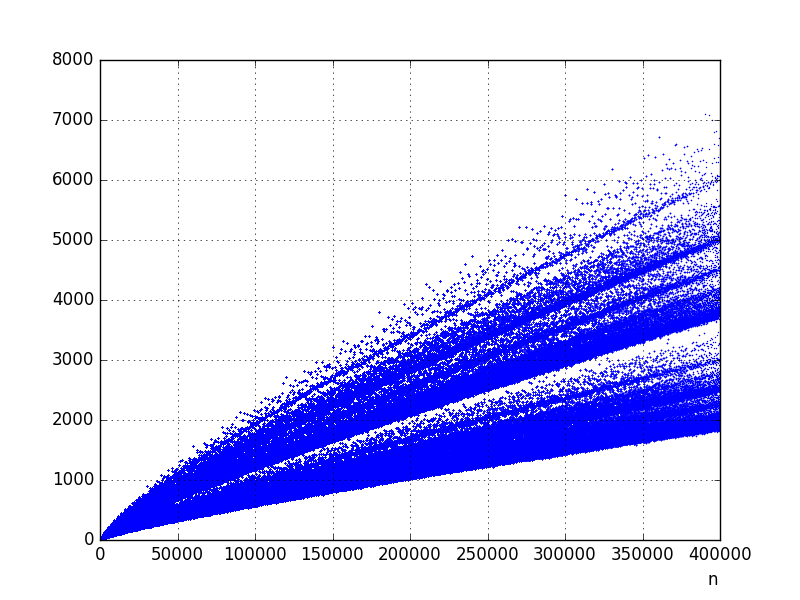
\includegraphics[width=9cm]{f_hypo_6kpm1}
\caption{ $R_{6k \pm 1}(n)$ ($4$ \textless $n$ \textless $2 \times 10^6$, $n = 2k, k \in \mathbb{N}$)}
\label{fig:6kmp1inpartitions}
\end{figure}

Conjecture (3) was confimed for $4 \leq m \leq 2 \times 10^6$ - this means that all even numbers $n$ that $8$ $\textless$ $n$ $\textless$ $4 \times 10^6$ have (3) fulfilled. Figure $\ref{fig:6kmp1inpartitions}$ depicts number of $GPs$ of even $n$ $\textgreater$ $4$ built from primes $p$ $\textgreater$ $3$. There is only one non-$6k \pm 1$-like prime which can be a member of such partition, $3$, but for s given $n$ it can be present in one $GP$ only (Lemma 1). This means that Figure $\ref{fig:6kmp1inpartitions}$ is very close to shape of original Goldbach's comet. \par
 \par

\begin{figure}[ht]
\centering
\captionsetup{justification=centering}
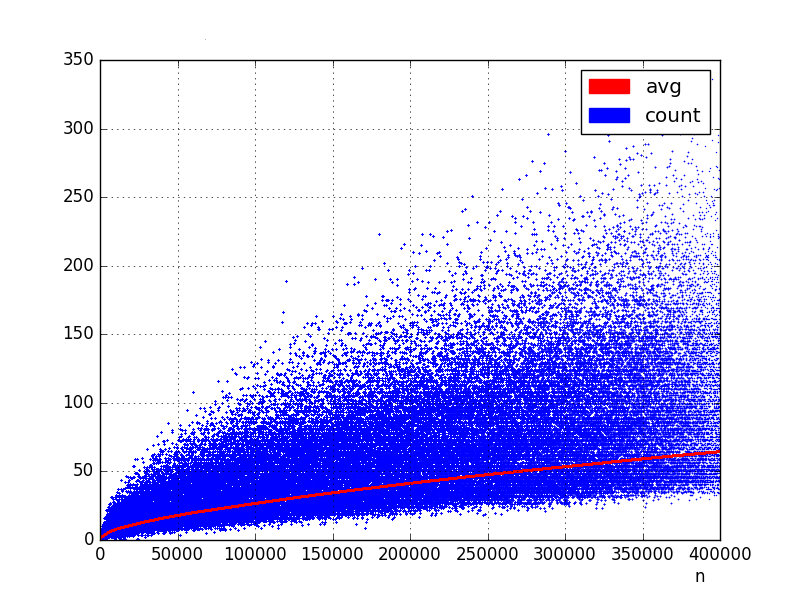
\includegraphics[width=9cm]{f_hypo_6km1_in_6n_4}
\caption{ Number of GPs  for $n$ with both primes that are the lesser of twin primes, with average values \\ ($n=4$ $mod$ $6$, $2$ \textless $n$ \textless $4 \times 10^5$, $n = 2k, k \in \mathbb{N}$)}
\label{fig:lessertwinprimesin6n4}
\end{figure}

\begin{figure}[ht]
\centering
\captionsetup{justification=centering}
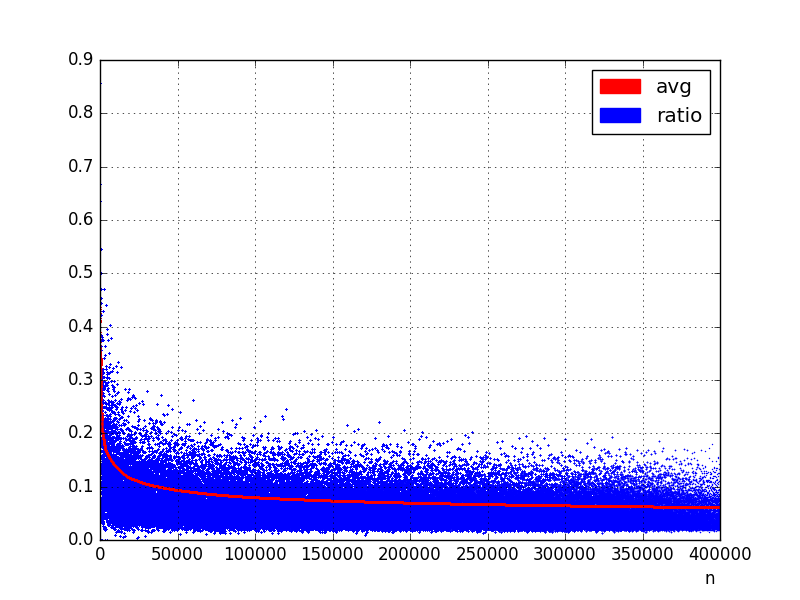
\includegraphics[width=9cm]{f_lesser_to_all}
\caption{ Ratio of $\left\vert R_{LTP}(n) \right\vert$ to $\left\vert R(n) \right\vert$, with average values ($n=4$ $mod$ $6$, $2$ \textless $n$ \textless $4 \times 10^5$, $n = 2k, k \in \mathbb{N}$)}
\label{fig:lessertwinprimesin6n4_to_all}
\end{figure}

Calculations run for $1 \leq n \leq 4 \times 10^6$ confirmed that there are only 12 known cases when even number of form $6n-2 \textgreater 2$ is not a sum of two the lesser of twin primes: 4, 94, 400, 514, 784, 904, 1114, 1144, 1264, 1354, 3244, 4204. This sequence was submitted to OEIS database as OEIS A321221 \cite{A321221}. $A$ in conjecture (4) is taken from last term: if $6n-2=4204$, then $n=701$, thus $A = 701$. A321221 is a subset of sequence A007534 \cite{A007534} described in \cite{zwillinger1979}. $701$ is also the last term of related sequence \cite{A243956}.\par

Figure $\ref{fig:lessertwinprimesin6n4}$ illustrates number of $GPs$ of $n$ ($4$ mod $6$) with two primes that are the lesser of twin primes. Let $R_{LTP}(n)$ be a set of all partitions of $n$ where both primes are the lesser of twin primes. Figure $\ref{fig:lessertwinprimesin6n4_to_all}$ depicts ratio of number of elements of $R_{LTP}(n)$ to number of elements of $R(n)$. Obviously this ratio is $0$ only for $n$ from OEIS A321221.\par

 It has been computationally verified that the following even numbers of form $6n-2$ have just one partition with two primes that are the lesser of twin primes: 10, 16, 28, 40, 52, 64, 106, 124, 136, 172, 184, 226, 262, 304, 394, 412, 442, 484, 544, 556, 604, 634, 664, 682, 694, 724, 736, 754, 772, 802, 874, 934, 976, 994, 1012, 1984, 1174, 1204, 1324, 1384, 1414, 1534, 1564, 1594, 1606, 1744, 1786, 1852, 1864, 1996, 2074, 2164, 2584, 2674, 3052, 3424, 3502, 3844, 9844, 12742, 15124, 15814, 24094, 24532 - no further terms were found so far. Figure $\ref{fig:lessertwinprimesin6n4}$ demonstrates ascending trend of average number of partitions of $6n-2$. \par
 
 Figures $\ref{fig:hypo6kpm1c1}$ and $\ref{fig:hypo6kpm1c2}$ are devoted to differences between primes of form $6k-1$ and $6k+1$ in GPs. In general we can observe two cases: the first one with difference close to 0, and the second one - with difference either positive or negative (and with generally ascending trend for bigger $n$).

\begin{figure}[ht]
\centering
\captionsetup{justification=centering}
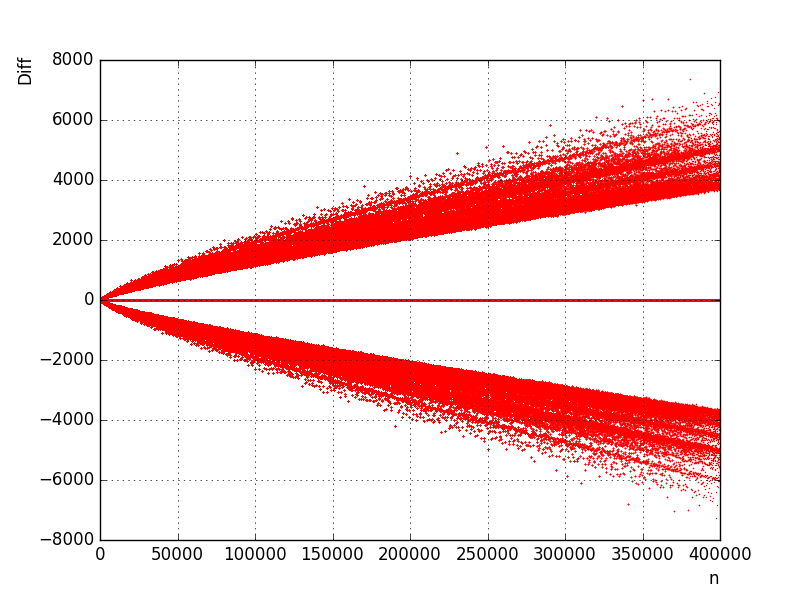
\includegraphics[width=9cm]{f_hypo_6kpm1_count1}
\caption{ Number of primes of form $6k-1$ in $R(n)$ - number of primes of form $6k+1$ in $R(n)$ ($2$ \textless $n$ \textless $4 \times 10^5$, $n = 2k, k \in \mathbb{N}$)}
\label{fig:hypo6kpm1c1}
\end{figure}

\begin{figure}[!ht]
\centering
\captionsetup{justification=centering}
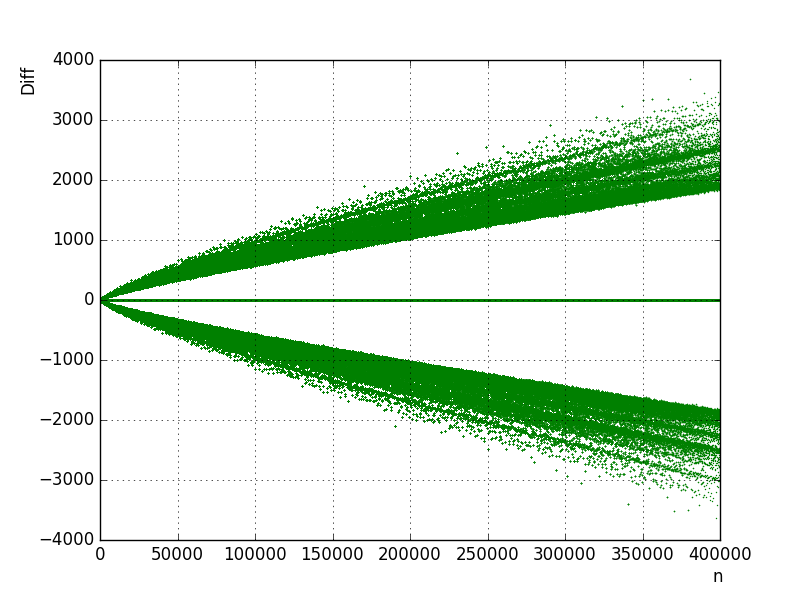
\includegraphics[width=9cm]{f_hypo_6kpm1_count2}
\caption{ $\left\vert R_{6k - 1}(n) \right\vert - \left\vert R_{6k + 1}(n) \right\vert$ ($2$ \textless $n$ \textless $4 \times 10^5$, $n = 2k, k \in \mathbb{N}$)}
\label{fig:hypo6kpm1c2}
\end{figure}

\section{Summary and next steps}

Executed experiments confirmed that (3) is true for $4 \leq n \leq 4 \times 10^6$ and (4) with $A=701$ is true at least for $1 \leq n \leq 4 \times 10^6$. As a result this work led to more precise conjecture (5):

\begin{equation}
\displaystyle\mathop{\bigforall}_{n \textgreater 701, n \in \mathbb{N}}
\displaystyle\mathop{\bigexists}_{p_1, p_2 \in \mathbb{P_{LT}}}
GSC(6n-2, p_1, p_2)
\end{equation}

If (5) is true, then $GSC$ is true.\par
Furthermore, even if $3$ looks to be the most common prime in GPs, executed experiments revealed that all even $n > 8$ have at least one partition without prime $3$, with both primes of form $6k \pm 1$. This observation raised another open question which can be foundation of further research work: which primes can be skipped in $GSC$? Maybe prime set is much bigger than required to fullfil $GSC$?

\begin{thebibliography}{9}
\bibitem{goldbach1742}
  Christian Goldbach, 
  \emph{On the margin of a letter to Leonard Euler},
  1742.
\bibitem{oliveira2012}
  Tomás Oliveira e Silva,
  \emph{Goldbach conjecture verification.}
  http://sweet.ua.pt/tos/goldbach.html,
  2012.
\bibitem{oliveira2013}
  Tomás Oliveira e Silva, Siegfried Herzog, and Silvio Pardi, 
  \emph{Empirical verification of the even Goldbach conjecture and computation of prime gaps up to 4 $\times 10^{18}$.}, 
  Mathematics of Computation, vol. 83, no. 288, pp. 2033-2060, 
  July 2014 (published electronically on November 18, 2013.
\bibitem{barylski2018}
  Marcin Barylski,
  \emph{Studies on Twin Primes in Goldbach Partitions of Even Numbers},
  http://tas-moto.org/research/TwinPrimesInGoldbachPartitions.pdf,
  2018.
\bibitem{A007528}
  OEIS Foundation Inc. (2018), The On-Line Encyclopedia of Integer Sequences, https://oeis.org/A007528. Primes of form 6n-1. 
\bibitem{A002476}
  OEIS Foundation Inc. (2018), The On-Line Encyclopedia of Integer Sequences, https://oeis.org/A002476. Primes of the form 6m+1.
\bibitem{A321221}
  OEIS Foundation Inc. (2018), The On-Line Encyclopedia of Integer Sequences, https://oeis.org/A321221. Numbers of the form 6n-2 which are not a sum of two numbers that are the lesser of twin primes.
\bibitem{A243956}
  OEIS Foundation Inc. (2018), The On-Line Encyclopedia of Integer Sequences, https://oeis.org/A243956. Positive numbers n without a decomposition into a sum n = i+j such that 6i-1, 6i+1, 6j-1, 6j+1 are twin primes.
\bibitem{A007534}
  OEIS Foundation Inc. (2019), The On-Line Encyclopedia of Integer Sequences, https://oeis.org/A007534. Even numbers that are not the sum of a pair of twin primes.
\bibitem{zwillinger1979}
  Dan Zwillinger,
  \emph{A Goldbach Conjecture Using Twin Primes}, Math. Comp. 33, No.147, p.1071, 
  1979.
\end{thebibliography}

\end{document}
